\documentclass[letterpaper]{article}
% Required Packages
\usepackage{aaai}
\usepackage{times}
\usepackage{helvet}
\usepackage{courier}
\usepackage{graphicx}
\usepackage{url}
\usepackage{multicol}
\usepackage{tabularx}
\usepackage{varwidth}
\usepackage{threeparttable}

\newcommand{\war}[1]{{\sf\small #1}}
%%%%%%%%%%
% PDFMARK for TeX and GhostScript
% Uncomment and complete the following for
% metadata if your paper is typeset using TeX and
% GhostScript (e.g if you use .ps or .eps files in your paper):
% \special{! /pdfmark where
% {pop} {userdict /pdfmark /cleartomark load put} ifelse
% [ /Author (John Doe, Jane Doe)
% /Title (Input Your Paper Title Here)
% /Subject (Input the Proceedings Title Here)
% /Keywords (Input your paper��s keywords here)
% /DOCINFO pdfmark
%}
%%%%%%%%%%
% PDFINFO for PDFTEX
% Uncomment and complete the following for metadata if
% your paper is typeset using PDFTEX
\pdfinfo{
/Title WikiTopics: What is popular on Wikipedia and why.
/Author Byung Gyu Ahn, Chris Callison-Burch, Benjamin Van Durme
/Subject AAAI-11
/Keywords Topic detection and tracking, Wikipedia
}
%%%%%%%%%%
% Section Numbers
% Uncomment if you want to use section numbers
% and change the 0 to a 1 or 2
% \setcounter{secnumdepth}{0}
%%%%%%%%%%
% Title, Author, and Address Information
\title{WikiTopics: What is popular on Wikipedia and why.}
\author{Byung Gyu Ahn
\and Chris Callison-Burch
\and Benjamin Van Durme\\
Center for Language and Speech Processing\\
Johns Hopkins University\\
Baltimore, Maryland\\
{\tt \{bahn, ccb, vandurme\}@cs.jhu.edu}}
%%%%%%%%%%
% Body of Paper Begins
\begin{document}
\maketitle

\begin{abstract}
We establish a novel task and pipeline to find trending topics from Wikipedia and introduce a novel data set:
hourly page view statistics of all Wikipedia articles for three years and evaluation data for the results.
Our pipeline consists of three steps: to find the best articles, cluster them, and extract the best sentences.
Our K-means clustering and clustering using the link structures performs with a 71.5\% precision compared to human annotators.
Our sentence selection make use of the link structure, named entity and time expression recognition and works 54\% as well as humans do.  
The result shows promise for explaining what is currently popular on Wikipedia and for automatically creating a timeline of past newsworthy events.
\end{abstract}

\section{Introduction}

%Recently, social media such as Twitter and Facebook gained attention from researchers.
%By looking at the topics recently prevailing in a lot of Twitter data at the same time, one may know the recent popular topics \cite{petrovic10}.

%Wikipedia has some relative advantage over Twitter as a source of topics, in that (1) it has a full description about the topic, (2) it has inter-article links that imply the relations between articles, and (3) the page view statistics are open to the public.

%The page view statistics are publicized in one of the wikipedians' website. Hour-by-hour statistics of size of 50-80Mbytes, each gzipped. The unzipeed file contains the project name, the article title, the page view counts, and the page size per line.

%\cite{ldc04} describes the definition of topics and events used in the TDT dataset. 

%* System overview describing each module, and including a diagram of how they connect (1.5 pages)
 %- include description of hour-by-hour wikipedia page view stats
   %+ show example graphs that highlight trending topics

%We first discuss previous work related to our work (\S2), then discuss our experimental design (\S3), and move on to show our experimental result (\S4). We then discuss our future work (\S5).

%There is an open-source software called Trending Topics (\url{http://www.trendingtopics.org/}) that shows the recent popular topics extracted from Wikipedia. We employed the same algorithm, which sorts the topics by the difference between the sum of the page counts of the recent 15 days and the sume of the page counts of the previous 15 days. Then, we picked the 100 topics of the highest differences.

In this paper we analyze a novel data set: we have collected the hourly page view statistics for every Wikipedia page in every language for a three year period.
We show how these page view statistics--along with a whole host of other features like inter-page links, edit histories, mentions in contemporaneous news stories--can be used to identify and explain popular trends, including political elections, natural disasters, sports championships, popular films and music, and other current events.

Our approach is to select a set of articles whose daily page views increase above their average from the previous two week period.
Rather than simply selecting the most popular articles for a given day, this selects articles whose popularity is rapidly increasing.
These popularity spikes are presumably due to some external current events in the real world.
On any given day, there are many articles whose popularity is spiking:
while some of articles are related to each other, many of them are a concidence.

In this paper we attempt to select 100 such articles from each of 5 randomly selected days in 2009
and cluster the articles such that the clusters coherently correspond to current events.
Quantitative and qualitative analyses are provided along with the evaluation data set.

We compared our automatically collected clusters to the Wikipedia current events.
Wikipedia editors compile current events every day, which mainly consist of social and political events,
traffic accidents and disasters. More often than not, they do not generate much traffic,
and link to pages that are too general like ``United States'' or ``Israel''.
We view this work as an automatic mechanism that could potentially supplant
the hand-curated method of selecting current events that is currently done by Wikipedia editors.

\begin{figure}
\centering
\begin{tabular}{|c|}
\hline
\war{Barack Obama} \\
\war{Joe Biden} \\
\war{White House} \\
\war{Inauguration} \\
\dots \\
\war{US Airways Flight 1549} \\
\war{Chesley Sullenberger} \\
\war{Hudson River} \\
\dots \\
\war{Super Bowl} \\
\war{Arizona Cardinals} \\
\hline
\end{tabular}
\caption{The automatically selected articles for January 27th, 2009. The underscores are used in place of spaces by Wikipedia.}
\label{fig:topics-jan-27}
\end{figure}

For instance, we would attempt to cluster the articles in Figure~\ref{fig:topics-jan-27} into 3 clusters, \{ \war{Barack Obama}, \war{Joe Biden}, \war{White House}, \war{Inauguration} \} which corresponds to the inauguration of Barack Obama, \{ \war{US Airways Flight 1549}, \war{Chesley Sullenburger}, \war{Hudson River} \} which corresponds to the successful ditching of an airplane into the Hudson river without loss of life, and \{ \war{Superbowl}, \war{Arizona Cardinals} \} which describes the then upcoming Superbowl XLIII.

We further try to explain the clusters by selecting sentences from the revision of the Wikipedia articles on that date. For the first cluster, a good selection might be ``the inauguration of Barack Obama as the 44th president of the United States took place on Jan 20, 2009''. For the second cluster, ``Chesley Burnett ``Sully'' Sullenberger III (born January 23, 1951)  is an American commercial airline pilot, \ldots, who successfully carried out the emergency water landing of US Airways Flight 1549 on the Hudson River, offshore from Manhattan, New York City, on January 15, 2009, \ldots.''. For the third cluster, ``[Superbowl XLIII] will feature the American Football Conference champion Pittsburgh Steelers (14-4) and the National Football Conference champion Arizona Cardinals (12-7) .'', which makes clear the relationship with \war{Arizona Cardinals}.

To generate the clusters we can make use of the text of the articles on that date, versions of the articles from previous dates, the link structure and category info from Wikipedia, and potentially external info like newspaper articles published before the date.

To select sentences we may want to make use of NLP technologies such as coreference resolution, named entity and date taggers, and dependency parsers to identify subjects of sentences.

\section{Motivation}

\begin{figure}
\centering
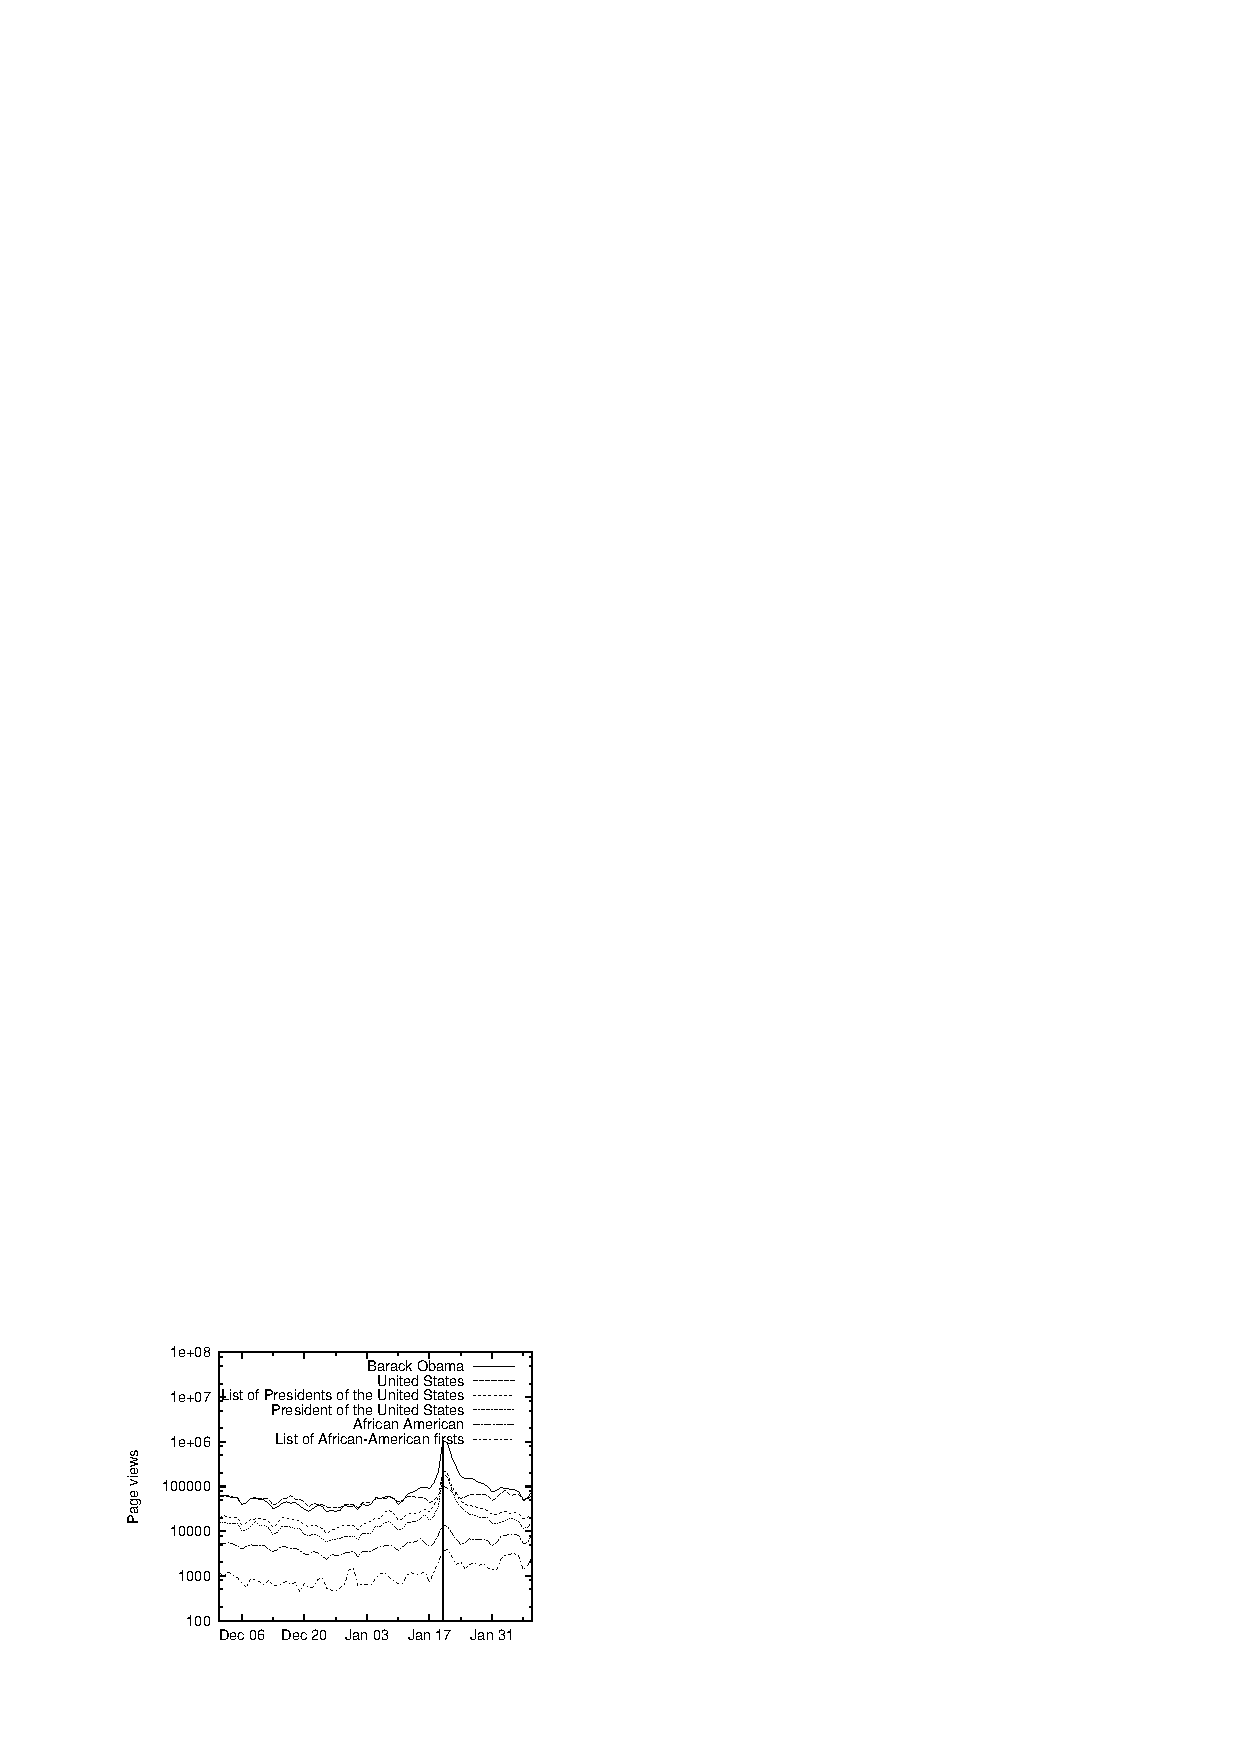
\includegraphics[width=0.5\textwidth]{figures/obama.pdf}
\caption{Page views for the articles related to the inauguration of Barack Obama. The articles are linked from an item in the Wikipedia current events. Interestingly, the list does not include the article \war{Inauguration of Barack Obama}, the very page about the event that has a spiking page views.}
\label{fig:obama-sparkline}
\end{figure}

What are interesting topics? In an online encyclopedia such as Wikipedia, the page view counts for each article reflects the popularity of the article. Each article has a different level of popularity: some have high page views, and others low page views. This tendency maintains throughout the year, but sometimes, a external newsworthy event such as a major political or sports event, a natural disaster or a pandemic, occurs and incur that many articles related to that specific event has a significant increase in page views.

Wikipedia has a section called ``current events'', in which the recently occurred events are listed manually by Wikipedia editors.
Figure~\ref{fig:obama-sparkline} shows the page views of the articles related to the inauguration of Barack Obama, as are manually listed in the Wikipedia current events section.
Each event may have a hierarchical structure--there may be a major event and minor events related to the major events.
Each event is described in a line of text with a possibly multiple links to the related Wikipedia articles.
The figure shows the spikes in page views of the related articles around the date on which the event took place--January 20th, 2009.

We set up a website\footnote{See \url{http://ANONYMIZED}.} that you can see the sparkline
graphs of pageviews for each day, each link, or each event in the form as Figure~\ref{fig:obama-sparkline}.
You can see the clear correlation between the spikes of the page views of the articles and the date on which the articles appear as the current events.

Following Trending Topics\footnote{See \url{http://www.trendingtopics.org}.}, we automatically select 100 articles for each day in 2009. The articles are selected based on the changes in page views for the previous 30 days, to detect a spike in page views. We refer to these articles are refered to as the WikiTopics articles.

We compared the automatically selected articles to the articles linked from the Wikpedia current events.
When evaluated against the articles linked from the Wikipedia current events, the WikiTopics articles perform badly with precision of 0.13 and the recall of 0.28.
There are two main reasons for this.
First, note that the hand-curated articles are less than half of the automatically selected articles:
There are 17,253 hand-selected articles and 36,400\footnote{The year 2009 has 365 days and one day is missing from our daily statistics.} WikiTopics articles.
Second, many of the hand-selected articles turned out having very low page views:
6,294 articles (36.5\%) have maximum daily page views less than 1000 in 2009.
Naturally, they are not chosen by automatic selection based on page views\footnote{The automatically selected articles has an increase in page views of at least 10,000.}.

Figure~\ref{fig:comparison-articles} shows the comparison of the selected articles.
Automatically selected articles include an newly created article about a politcal event
(\war{Inauguration of Barack Obama}), a recently released film, a popular TV series and
related articles and tend to be specific than hand-selected articles.
The hand-selected articles include more generic articles related a specific event,
most of which are personal, organizational or geopolitical names.
The hand-generated event describes the relationships between related articles.

Should we try to predict the current events descriptions
that Wikipedia editors hand-curate? We say no for the following reasons.
They are not interesting topics: many of them have too low page views,
which does not draw people's attention.
Also, the hand-curated articles are too generic and biased to geopoltical names
such as the names of countries.
Therefore we recommend against this methodology for other researchers.

we establish a more concrete goal of our novel task:
to detect recent events from popular Wikipedia articles,
summarize the events, and provide the links to the relevant Wikipedia articles
just as the hand-curated Wikipedia current events do,
except that the events are popular topics that have a significant increase in
page views. This work can be used to replace the hand-curated Wikipedia current events,
listing the events that in reality many people are interested in.

\begin{figure}
\centering
\begin{tabular}{c}
WikiTopics \\
\hline
\war{Inauguration of Barack Obama} \\
\war{Joe Biden} \\
\war{Notorious (2009 film)} \\
\war{The Notorious B.I.G.} \\
\war{Lost (TV series)} \\
ldots \\
\\
Wikipedia current events \\
\hline
\war{Fraud} \\
\war{Florida} \\
\war{Hedge fund} \\
\war{Arthur Nadel} \\
\war{Federal Bureau of Investigation} \\
\end{tabular}
\caption{ The example articles for January 27th. These are the articles that do not have a counterpart with a window size of 15 days. The hand-selected articles are linked from an event ``Florida hedge fund manager Arthur Nadel is arrested by the United States Federal Bureau of Investigation and charged with fraud.'' \\ }
\label{fig:comparison-articles}
\end{figure}

%Some of the most charateristic instances from the topics and the events are shown in Table~\ref{tab:topics-events-comparison}.
%We evaluated the precision and recall score of the TrendingTopics topics against the Wikepedian Current Events (Table~\ref{tab:topics-events-evaluation}.
%Their precision and recall scores are extremely low.
%Probably, wikipedians are more interested in political and scientific topics,
%and the page view statistics tend to be more dramatic for the societal and cultural events--recent deaths of famous people,
%recent release of movies and music albums.

%We have selected the articles with more page views above the previous two weeks.
%\cite{petrovic10}
%What are interesting topics? This could be an aesthetic question, but, in Wikipedia,
%gaining popularity usually means a big inflow of users looking up an article of a specific topic.
%More often than not, a popular on-going event accompanies many topics, or Wikipedia articles,
%collecting sudden increases in page view counts (Figure~\ref{fig:topics-for-an-event}).
%The TrendingTopics algorithm (\S\ref{sec:related-work}) finds a big increase in page view counts and make a list of the articles with the highest increase. 

%Due to the discrepancy between the Wikipedian Current Events and the topics based on page views,
%it was not realistic to predict from the page view counts the topics that would overlap the Current Events.
%We set the topics extracted by the TrendingTopics algorithm as the baseline data.

%Figure~\ref{fig:process} outlines the subprocesses discussed in this paper. The first phase, {\it topic selection} is the step that 

Our system pipeline and this paper are organized as follows. First, the most popular articles are collected per each day (\S\ref{sec:article-selection}). Second, correlated articles are clustered into the clusters that correspond to intersting events or topics (\S\ref{sec:clustering}). Lastly, the sentence that best describes the interesting events are extracted (\S\ref{sec:textualization}). See the process diagram in Figure~\ref{fig:process}.

\begin{figure*}
\centering
\includegraphics[width=0.9\textwidth]{figures/WikiTopicsPipeline.pdf}
\caption{Process diagram.
(a) Topic selection: select interesting articles based on increase in page views.
(b) Clustering: cluster the articles according to relevent events using K-means or the link structure.
(c) Textualization: select the sentences that best summarizes the relevant events in text. }
\label{fig:process}
\end{figure*}

\section{Article selection}
\label{sec:article-selection}
\paragraph{Dataset}
The Wikipedia Traffic Statistics dataset is originally made available\footnote{See \url{http://dammit.lt/wikistats}.} by a Wikipedian Domas Mituzas.
This data is only kept up to a several months that the space allows.
For the previous statistics, two sets of the statistics are published at Amazon Public Datasets\footnote{See \url{http://aws.amazon.com/datasets/2596} and \url{http://aws.amazon.com/datasets/4182}.}).
This dataset consists of the files that each has hourly page view statistics for every article in every language.
Each line of the files contains the language or the project name, the title, the hourly page views, and the numbers of bytes of the text of an Wikipedia article.
We limited the work only to the English Wikipedia.

\paragraph{Preprocess}
These statistics are collected from the Wikipedia cache server as requested by users, and it includes many wrongful or malicious requests.
Many requested pages are also redirect pages that automatically refer the requester into another page.
The redirect pages are usually the ones that are different names of an entity.
To process these difficulties, we downloaded the English Wikipedia dump on June 22nd, 2010 from Wikimedia dump\footnote{See \url{http://download.wikipedia.org}.} and from the database dump extracted the list of the titles of all articles and the redirect articles.
Using these data, we filtered out the request for non-existing articles and merged the page views for the redirect pages into the main articles.
Also the title of the Wikipedia articles has to be normalized according to a specific format, that is, the first letter of each title are capitalized and a space in it has to be replaced with an underscore, and so on.

\paragraph{Design}
For each day, the 100 articles with the most increase in page views are selected.
The difference between the total sum of page views for the past 15 days
and the total sum of page views for the previous 15-days period are calculated,
and the articles are sorted in the order of decreasing difference.
To facilitate the process, the articles with too small page views are ignored.

\paragraph{Evaluation}
We do not attempt to evaluate the selected articles against the Wikipedia current events for the reasons in the previous section.

\section{Clustering}
\label{sec:clustering}

More often than not, more than one popular articles are related to an external current event.
For example, all the hand-selected articles shown in Figure~\ref{fig:comparison-articles}
are related to a Wikipedia current event that ``Florida hedge fund manager Arthur Nadel is arrested \ldots and charged with Fraud.''
Among the automatically selected articles, main events such as \war{Inauguration of Barack Obama} and release of the file \war{Notorious (2009 film)} involves making popular the incidental articles about the players of the events such as \war{Joe Biden} and \war{The Notorious B.I.G.} along with the articles about the main events themselves.

We attempt to cluster the automatically selected articles into mutually related articles and find the article that describes the main event for each cluster. For clustering, we make use of the unigram bag-of-words model and the link structures of articles. To find the centroid articles that describes the main event, we used K-means model and the link structure of articles.

\paragraph{Dataset} For each day of the five selected dates in 2009,
we downloaded the text of the 100 automatically selected articles from Wikipedia.
The downloaded texts are the latest texts as of the date on which the article is selected.
We use the Wikipydia module, which is a python module to make use of the Wikipedia API.
As preprocessing, we stripped out all HTML tags from the article text, and
replaced the Wikipedia-specific tags as the corresponding text using the mwlib\footnote{See \url{http://code.pediapress.com/wiki/wiki/mwlib}.} library,
and finally split sentences using NLTK \cite{Loper02NLTK}.

\paragraph{Design}
As a baseline, two different clustering scheme makes use of the link structure: \textsc{CompConn} and \textsc{OneHop}.
\textsc{ConnComp} is to cluster articles in the same connected components, connecting articles that have a direct link from one to another.
\textsc{OneHop} is to cluster articles within only one hop.
The number of resulting clusters depend on the order in which you choose the next article to cluster.
To find the minimum number of such clusters is NP-complete.
Instead of attempting to find the optimal clusters,
we just tried to cluster in the descreasing order of the number of links: With most links, first clustered.
The link structure is downloaded from the website of Henry Haselgrove\footnote{See \url{http://users.on.net/~henry/home/wikipedia.htm}.}.

We also perforemd K-means clustering on the set of articles, treating the article texts as bag of words.
For 100 automatically selected articles on each of the five selected dates,
the number of clusters $K$ was set to 50.
We used the Mallet \cite{McCallumMALLET} software to run K-means clustering.
Normalization and tokenization are not performed before running K-means.
The algorithm calculates the mean of each cluster in word-vector space,
and we chose the centroid article that is closest to the center in the vector space.

\paragraph{Evaluation}
Three annotators performed manual clustering on the topics for the five specified dates to get the gold standard clusters.
The three manual clusters were evaluated against each other to measure the annotator agreement,
using the multiplicity B-cubed metric \cite{amigo09} that can handle overlapping clusters.
The results are shown in Table~\ref{tab:clustering-results}.

\begin{table}
% table from /Users/bahn/Dropbox/Documents/Research/Wikitopics/Clustering\ Accuracy.xlsx
% CCB is Manual-1, Ben Manual-2, and Byung Manual-3.
\centering
\begin{tabular}{ccc}
Test set & Gold standard & B-Cubed F-score \\
\hline
\textsc{Manual-1} & \textsc{Manual-2} & 0.735 $\pm$ {\small 0.085} \\
\textsc{Manual-1} & \textsc{Manual-3} & 0.672 $\pm$ {\small 0.076} \\
\textsc{Manual-2} & \textsc{Manual-3} & \textbf{0.747} $\pm$ {\small 0.129} \\
\hline
\hline
\textsc{ConnComp} & \textsc{Manual-1} & 0.302 $\pm$ {\small 0.122} \\
& \textsc{Manual-2} & 0.342 $\pm$ {\small 0.134} \\
& \textsc{Manual-3} & 0.397 $\pm$ {\small 0.068} \\
\hline
\textsc{OneHop} & \textsc{Manual-1} & 0.395 $\pm$ {\small 0.151} \\
& \textsc{Manual-2} & 0.468 $\pm$ {\small 0.170} \\
& \textsc{Manual-3} & 0.476 $\pm$ {\small 0.147} \\
\hline
\textsc{K-means}& \textsc{Manual-1} & \textbf{0.534} $\pm$ {\small 0.034} \\
& \textsc{Manual-2} & \textbf{0.534} $\pm$ {\small 0.050} \\
& \textsc{Manual-3} & 0.494 $\pm$ {\small 0.035} \\
\hline
\end{tabular}

\caption{Clustering evaluation. \textsc{ConnComp} and \textsc{OneHop} are clustering using the link strcuture.
\textsc{K-means} clustering uses the text of the articles as bag of words.
For the B-Cubed metric, exchanging the gold standard and the data set results
in the exchange of the precision and the recall score, thus leaving the F-score same.}
\label{tab:clustering-results}
\end{table}

The B-cubed metric is one of the extrinsic clustering evaluation metrics, which need a gold standard set of clusters to evaluate the set of clusters of interest against.
Each item $e$ has potentially multiple gold standard categories, and also potentially multiple clusters.
Let $C(e)$ is the set of the clusters that $e$ belongs to, and $L(e)$ is the set of $e$'s categories.
The multiplicity B-cubed scores for a pair of $e$ and $e'$ are evaluated as follows:

$$ \mbox{Prec}(e,e') = { \min \left( |C(e) \cap C(e')| , |L(e) \cap L(e')| \right) \over |C(e) \cap C(e')| } $$
$$ \mbox{Recall}(e,e') = { \min \left( |C(e) \cap C(e')| , |L(e) \cap L(e')| \right) \over |L(e) \cap L(e')| } $$

The overall B-cubed scores are evaluated as follows:

$$ \mbox{Prec} = \mbox{Average} _{e \neq e'} \mbox{Prec}(e,e') $$
$$ \mbox{Recall} = \mbox{Average} _{e \neq e'} \mbox{Recall}(e,e') $$

The inter-annotator agreement in the B-cubed scores are in the range of 0.672-0.747.
Clustering with the link structure performed the worse, having half of the precision
for manual clusters.
K-means clustering performs best, achieving 71.5\% precision compared to 
manual clustering.

\paragraph{Analysis}

There are two main reason that the link structure performed worse.
First, the link structure was too old. The link structure was generated on
January 28, 2009 and 13.2\% of the WikiTopics articles were created after the date,
thus missing from the link structure. Second, there are a few ``octopos'' articles
that have links to many articles, and group them into one large cluster.
\war{The United States} on January 27, 2009 was particularly harmful,
grouping 79 articles into a single cluster.

\textsc{K-means} has its own defects: it does not distinguish different meanings of words.
For example, the automatically selected articles for April 19 include
both \war{Piracy in Somalia} and \war{The Pirate Bay} as well as \war{Piracy}.
Their resemblance in word spelling might result in confusion in clustering,
depending on the clustering method.
In fact, \textsc{K-means} correctly clustered \war{The Pirate Bay} with \war{The Pirate Bay Trial},
but clustered \war{Piracy} with \war{USS Bainbridge (DDG-96)} and \war{MV Maersk Alabama},
both of which are the names of vessels.
Instead of \war{Piracy}, \war{Moldova} wrongfully ended up in the same cluster as \war{Somalia} and \war{Piracy in Somalia}.
In contrast, clustering method using the link strcuture, \textsc{CompConn} and \textsc{OneHop} correctly clustered
\war{Somalia}, \war{Piracy in Somalia}, and {Piracy} all in the same cluster.

Clustering the articles according to the relevance to recent popularity is not a trivial work
even for humans. In automatically selected articles for February 10, 2009,
\war{Journey (band)} and \war{Bruce Springsteen} may seem to be relevant to \war{Grammy Awards},
but in fact they are relevant on this day because of the \war{Super Bowl}.
The \textsc{K-means} clusters wrongfully merged the articles relevant to \war{Grammy Awards} or \war{Super Bowl}
into a cluster.

\section{Textualization}
\label{sec:textualization}

We attempt to generate textual descriptions for the clustered articles to explain why they are popular and what event is relevant.
We consider the date expressions, the reference to the article as features. Currently, our work is limited to
select the best sentence that describes the relevant events,
but it could be future work to descibe the relationships of the articles to the relevant event,
and summarize the description using sentence fusion or paraphrasing.
Often, some articles are directly connected to an external event
while others are subsidiary topics that show vague connection.

%Specifically, the textual description for each cluster may consist of the sentences (1) that describe why the cluster is popular at the time and (2) that describe why each topic in the cluster is popular.
%The concepts of central and peripheral topics (\S\ref{ssec:clustering}) are important in that different types of topics contribute to the description in different ways.
%Often, the central topics are directly related to the event that caused the recent popularity and often includes a direct explanation of the recent event. 

\paragraph {Preprocess}
We preprocess the Wikipedia articles using the SERIF system \cite{BoscheeSerif} for date tagging and coreference resolution.
The identified temporal expressions are in various formats such as exact date (``February 12, 1809''), a season (``spring''), a month (``December 1808''), a date without a specific year (``November 19''), and even ralative time (``now'', ``later that year'', ``The following year''). Some examples are showed in Figure~\ref{fig:temporal-expressions-examples}.
The coreferences are analyzed into a list of the entities in the article and all the mentions of each entity in the article are compiled as co-ref chains.

\begin{figure}
\centering
\begin{multicols}{2}
%\begin{tabular}{|c|}
%\hline
February 12, 1809 \\
1860 \\
now \\
the 17th century \\
some time \\
December 1808 \\
34 years old \\
spring \\
September \\
Later that year \\
about 18 months of schooling \\
November 19 \\
that same month \\
The following winter \\
The following year \\
April 1865 \\
late 1863 \\
\end{multicols}
\label{fig:temporal-expressions-examples}
\caption{Examples of temporal expressions identified by the SERIF system in the preprocess step,
selected from 247 such date and time expressions extracted from the article \war{Abraham Lincoln}.}
\end{figure}

\paragraph {Design}
As a baseline, we picked the first sentence for each article because the first sentence generally explains the article.
The first sentence usually summarizes the topic of the article and is often relevant to the external event.
We refer to this as \textsc{First}.

As a second baseline, we picked the sentence with the most closest date to the date on which the article was selected.
Closeness refers to the difference in days between the dates.
The dates in sentences could vary in their formats, so we put precedence over the formats so that
more exact date i.e. ``Feburary 20, 2009'' has precedence over more vague date formats such as ``February 2009'' or ``2009''.
We refer to this scheme as \textsc{Recent}.

For the third data set, we picked the sentence both with the most recent date and with the reference to the article's topic.
We refer to this sceme as \textsc{Self}.

After selecting a sentence for each cluster, we used coreference resolution to substitute personal pronouns in the sentence with their proper names.
This step enhances readability of the selected sentence, which often refers to its subject by a pronoun such as ``he'', ``his'', ``she'', or ``her'.
The examples of substituted proper names appear in Figure~\ref{fig:sentence-selection} in bold face.

\begin{figure*}
\begin{tabularx}{\linewidth}{cX}
2009-01-27 & \war{Abraham Lincoln} \\
\textsc{Sent} & \small To commemorate his upcoming 200th birthday in February 2009, Congress established the Abraham Lincoln Bicentennial Commission (ALBC) in 2000. \\
\textsc{Coref} & \small To commemorate \textbf{Lincoln's} upcoming 200th birthday in February 2009, Congress established the Abraham Lincoln Bicentennial Commission (ALBC) in 2000. \\
\hline
2009-01-27 & \war{Barack Obama} \\
\textsc{Sent} & \small He was inaugurated as President on January 20, 2009.\\
\textsc{Coref} & \small \textbf{Obama} was inaugurated as President on January 20, 2009.\\
\hline
2009-02-10 & \war{Michael Phelps} \\
\textsc{Sent} & \small His second book, No Limits: The Will to Succeed, was released on December 9, 2008.\\
\textsc{Coref} & \small \textbf{Phelps's} second book, No Limits: The Will to Succeed, was released on December 9, 2008.\\
\hline
2009-05-12 & \war{Eminem}\\
\textsc{Sent} & \small He is planning on releasing his first album since 2004, Relapse, on May 15, 2009.\\
\textsc{Coref} & \small \textbf{Eminem} is planning on releasing his first album since 2004, Relapse, on May 15, 2009.\\
\end{tabularx}
\label{fig:sentence-selection}
\caption{Selected examples of sentence selection and coreference resolution.
From each \war{article} the best \textsc{sent}ence is selected
based on the most recent date expression and the reference of the topic,
and the personal pronouns are substituted with their proper names,
which are typed \textbf{bold}.}
\end{figure*}

The SERIF system finds the chain of coreference and tags the type of each reference
as proper name, nominal position, or pronoun.
There may be more than one proper name for each chain and to choose the best one
is not a trivial task: proper names vary from \textit{John} to \textit{John Kennedy} to \textit{John Fitzgerald ``Jack'' Kennedy}.
Our algorithm chose the most frequent proper name to substitute with.

\paragraph {Evaluation}
For ten articles on each of five selected dates, an annotator selected sentences that describes why each article gains in popularity,
among 289 sentences per each article on average.
The annotator picked the one best sentence, and the possible multiple second best sentences.
In the case there are no best sentence among them, he marked none as the best sentence,
and listed all the partially explaning sentence as second best sentencess.

To see inter-annotator agreement, another annotator selected the best sentence for the ten articles of the first date.

The evaluation results for all the selection schemes are shown in Table~\ref{tab:sentence-selection-results}.

\begin{table}
	\centering
	\begin{threeparttable}
		\begin{varwidth}{\textwidth}
			\begin{tabular}{cccc}
				Scheme & Prec\tnote{1} & Recall\tnote{1} & Prec\tnote{2} \\
				\hline
				\textsc{Manual}\tnote{3} & \small 0.63 & \small 0.83 & \small 0.75 \\
				\hline
				\textsc{First} & \small 0.14 & \small 0.21 & \small 0.34 \\
				\textsc{Recent} & \small \textbf{0.33} & \small \textbf{0.48} & \small \textbf{0.55} \\
				\textsc{Self} & \small \textbf{0.33} & \small \textbf{0.48} & \small 0.53 \\
			\end{tabular}
		\end{varwidth}
		\begin{tablenotes}\footnotesize
			\begin{varwidth}{\textwidth}
				\item[1]{ Evaluated against the best gold standard sentence. }
				\item[2]{ Evaluated against the best and secondary sentences. }
				\item[3]{ Evaluated for only the first date. }
			\end{varwidth}
		\end{tablenotes}
		\caption{The precision of different sentence selection scheme. Except for \textsc{Manual},
		all sentence scheme are evaluated for the five selected dates. }
		\label{tab:sentence-selection-results}
	\end{threeparttable}
\end{table}
\paragraph {Analysis}

\war{Serena Williams} is an example that the error in sentence splitting
propagates to the sentential selection. The best sentence manually selected
was the first sentence in the article ``Serena Jameka Williams \ldots
, as of February 2, 2009, is ranked World No. 1 by the Women's Tennis
Association \dots .'' The sentence was disastrously divided into two sentences
right after ``No.'' by the NLTK splitter through our preprocess.
It means no matter how well the sentential selection is done,
it cannot choose the gold standard sentence. We ran the splitta
\cite{dgillick09sbd} over the article text and found that it does not
split the first sentence at the wrong position. The better the splitting is,
The better the sentential selection works.

Selection of the best sentence with a \textsc{Recent} date seems to work well,
with some problems.  \war{Farrah Fawcett} is a nice example of multiple sentences
with dates, in a single section, that could potentially be spliced
together into a timeline (the final event, that she was released from
the hospital, makes more sense if we included why she was there).
Furthermore, the sentence describing the most recent event contains
a date without the year, which has less precedence over the other dates with the year
even when it is closer to the date of interest than the others are.
So having precedence over the date forms might not always work well.

The baseline, selection of the \textsc{First} sentence, performs badly,
but in 1/3 of the articles they are at least secondary articles, if not best.
It is because the first sentence is an overall introduction about the topic,
often including its recent achivement or a person's death.

The feature of selecting the sentence with a reference to the topic
must be used another feature such as \textsc{Recent} because
it is not comparable but a binary feature.

- summarizing/sentence fusion


%An improved baseline for sentence selection would include the opening
%sentence of the page from which the date-stamped sentence comes from.
%For example, in ``pick0419'' :
%
%\war{Grey Gardens} \# ``It is scheduled to air on HBO on April 18, 2009.''
%
%as compared to:
%
%\war{Grey Gardens} \# Grey Gardens is a 1975 documentary film by the
%direction/cinematography/editing team of Albert and David Maysles,
%Susan Froemke, Ellen Hovde, and Muffie Meyer. ...  It is scheduled to
%air on HBO on April 18, 2009.
%
%From there we'd want to compress the opening sentence, as in this case:
%
% \war{Grey Gardens} \# Grey Gardens is a 1975 documentary film. ...  It is
% scheduled to air on HBO on April 18, 2009.
%
% Which then brings up the potential flaw:  it is an *adaptation* of
% this film that is being released on April 18th, not the original.
%
% Looking deeper, we see the earlier sentence: ``Grey Gardens, a film for
% HBO, starring Jessica Lange and Drew Barrymore as the Edies, with
% Jeanne Tripplehorn as Jacqueline Kennedy, and Daniel Baldwin as Julius
% Krug.''.  This is hard: even if we run a co-ref system over the page to
% resolve the ``It'' in ``It is scheduled to air'', then we'll know that
% ``Grey Gardens'' is scheduled to to air.  But it isn't the same Grey
% Gardens, it is the new adaptation, which we know only from the section
% header.  Or we would have to have background knowledge that could
% enable reasoning about movies not having two different lists of
% starring actors, etc. (even harder!)


\section{Related work}
\label{sec:related-work}

There should be lots of citation to related work here. Examples are NewsBlaster by McKeown and Barzilay; Snippet Selection by Lapata, and a list of ACL/EMNLP papers that study wikipedia.

The similar approach was done by Newsblaster and NewsInEssence before. They were the systems that combine various human language techonologies into a pipeline.

Summarization was done by both the systems. Newsblaster used the ones...

Multilingual system was tried by Newsblaster. They first tried...



\section{Future work}

Each step of the WikiTopics system can be developed further.

First, article selection.
Should we predict what the Wikipedia current events will be?
No.
But if we can predict which will come next before any newspaper or traditional media, it would be awesome.
But should we be? The point is in automaticity anyway.
We currently use the absolute difference in page views with the window of size 15-days.
Using relative difference might be useful.

Second, clustering.
Hierarchical clustering... There a lot of clusters that have hierarchical structures. For example, on the day of the
inauguration of Barack Obama, the automatically selected articles include
the former presidents of the United States, family of Barack Obama,
and the appointed staff in the new goverment.
Using hierarchical clustering, the summary of each cluster will be better.

Third, sentence selection. Sentence fusion could be useful. Most of the Wikipedia current events 
contain more than two links to articles. We currently select one sentence per each article,
but it might be true sometimes that fewer sentences can well explain the events.
We can use hierarchical clustering to summarize the clusters with fewer sentences.

%\section*{Acknowledgments}

%The first author was supported by Samsung Scholarship.

%We appreciate Wikipedians Domas Mituzas and Fr\'{e}d\'{e}ric Schu\"{u}tz
%for making the page views statistics avaialble and Peter Skomoroch for
%prividing Trending Topics and answering questions.

% References and End of Paper
\bibliography{bahn}
\bibliographystyle{aaai}
\end{document}